\subsection{Symptomer}
KOL udvikles over mange år, dog bemærkes sygdommen ofte ikke før lungefunktionen er markant nedsat. Dette betyder, at KOL og dens symptomer som regel først kommer til udtryk efter $50$ årsalderen \cite{Lange2015}. Dette kan i praksis betyde, at patienter først opsøger en læge, når deres lungefunktion er halveret \cite{dsam2016}.

Symptomer på KOL opleves som åndenød og hoste ved fysisk aktivitet. Hosten er ofte med ekspektoration, som hos de fleste patienter er klart eller hvidt.\cite{Basisbogen2016} Derudover er der en tendens til hyppig eksacerbationer, hvilket er tilfælde, hvor KOL-patienters tilstand akut forværres og kræver behandling. Eksacerbationer forekommer hyppigere som KOL udvikler sig, og kan tage op til flere uger før patienten ikke længere er påvirket af eksacerbationen \cite{Anzueto2010}. KOL-patienter klassificeret med moderat KOL af \autoref{tab:GOLD} oplever i gennemsnit 2,68 eksacerbationer pr. år, mens patienter med svær KOL oplever 3,43 eksacerbationer pr. år \cite{Anzueto2010}.
Symptomerne i forhold til eksacerbationer opleves som øget åndenød, hoste samt grønt eller gulligt ekspektoration og øget purulens. Denne tilstand skyldes ofte bakterielle infektioner, hvilket udgør ca. halvdelen af tilfældene.\cite{dsam2016,Basisbogen2016} 

Der er en række komorbiditeter, som hyppigt ses hos KOL-patienter, der kan have en negativ påvirkning på patienters livskvalitet og prognose. Derfor bør patienter regelmæssigt tjekkes for de hyppigste komormiditeter, såsom kardiovaskulære sygdomme, type-2 diabetes, osteoporose, lungecancer, muskelsvækkelse samt angst og depression.
Nogle af komorbiditeterne kan skyldes, at åndenød har medført et nedsat fysisk aktivitetsniveau og dermed svage perifere muskler samt vægttab \cite{dsam2016}. Desuden har tobaksrygning og generelt dårlig livsstil betydning for udviklingen af disse komorbiditeter.\cite{dsam2016, McCarthy2015}
Psykiske komorbiditeter, ofte i form af depression og angst, har en øget forekomst hos patienter med en FEV1 værdi på under 50 \% af den forventede værdi. Den øgede risiko for psykiske lidelser skyldes, at KOL kan medføre social isolation og tab af sociale relationer, skyldfølelse og usikkerhed i forhold til fremtiden.\cite{dsam2016}


\subsection{Diagnose}
Ved mistanke om KOL undersøges lungefunktionen ved spirometrimålinger, hvor FEV1 og FVC måles. Af \autoref{fig:FEV} ses spirometrimålinger for henholdsvis patienter med normal og obstruktiv nedsat lungefunktion samt en kombination af disse.\cite{Basisbogen2016, Sundhed2013}

\begin{figure} [H]
\centering
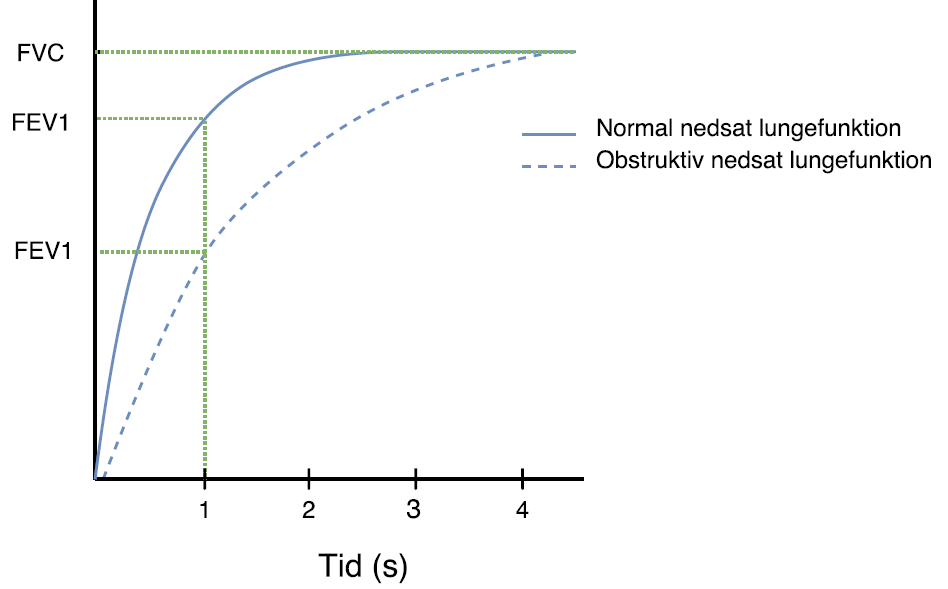
\includegraphics[width=0.8\textwidth]{figures/FEV}
\caption{Spirometrimålinger for patienter med normal og obstruktiv nedsat lungefunktion. Revideret\cite{Basisbogen2016}.}
\label{fig:FEV}
\end{figure} 

\noindent
Det fremgår af \autoref{fig:FEV}, at der ved obstruktivt nedsat lungefunktion er et fald i FEV1 samt FVC. Der udføres ligeledes en reversibilitetstest for at sikre, at patienter ikke lider af differentialdiagnosen astma. Disse patienter gives broncodilatorer, som hos astmapatienter vil forbedre spirometrimålingen, mens lungefunktionen for KOL-patienter forbliver uændret.\cite{Basisbogen2016, Sundhed2013} 
For at undersøge KOL og patienters komorbiditeter undersøges foruden lungefunktionsundersøgelser også BMI, røntgen af thorax, EKG-målinger og blodprøver \cite{Sundhed2013}. 
%Med tiden kan symptomerne på KOL forværres, og der skal mindre fysisk aktivitet til for at udløse åndenød. \cite{Basisbogen2016}